
\begin{frame}
  \frametitle{Making useful XANES calculations}

  The challenge to using \textsc{feff}8 \textit{well} is that you need
  to provide a list of atomic coordinates.  But if you already know
  where the atoms are, you probably don't need to calculate the XANES.

  \bigskip

  In this section, we will briefly discuss how to handle

  \begin{itemize}
  \item Vacancies and substitutions
  \item Structural distortions
  \end{itemize}

  We will also discuss
  \begin{itemize}
  \item \textsc{feff}'s concept of computing {\color{Blue4}self
      consistent potentials}
  \item {\color{Blue4}Fitting} XANES spectra as implemented in
    \textsc{mxan} and \textsc{FitIt}.
  \end{itemize}
\end{frame}

\begin{frame}
  \frametitle{Vacancies and substitutions}
  \begin{itemize}
  \item In \textsc{feff}, a point in space is occupied by {\color{Blue4}one
      or zero} atoms and may not be partially vacant or fractionally
    occupied.
  \item These effects cannot be computed by a \alert{single}
    \textsc{feff} calculation.
  \item The most successful strategy is to make multiple calculations,
    randomly introducing substitutions or vacancies.
  \item Sum these calculations progressively until the average is
    converged.
  \item Convergence will probably happen within 10 or 20 calculations.
  \end{itemize}
\end{frame}

\begin{frame}
  \frametitle{Structural distortion}
  \begin{columns}
    \begin{column}{5cm}
      \centering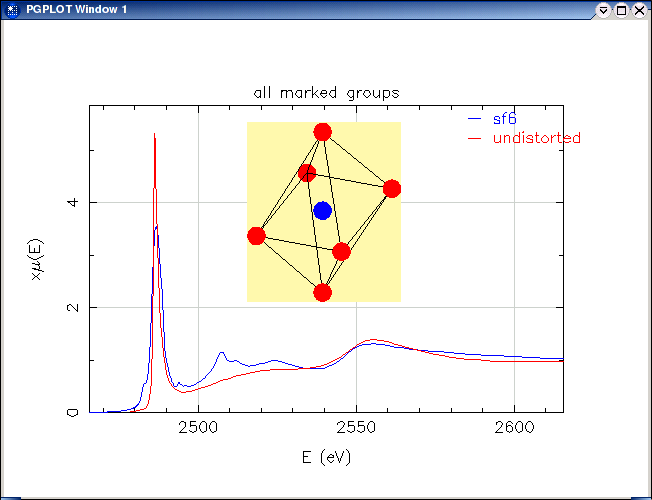
\includegraphics[width=0.9\linewidth]{images/SF6/sf6_undistorted}

      \centering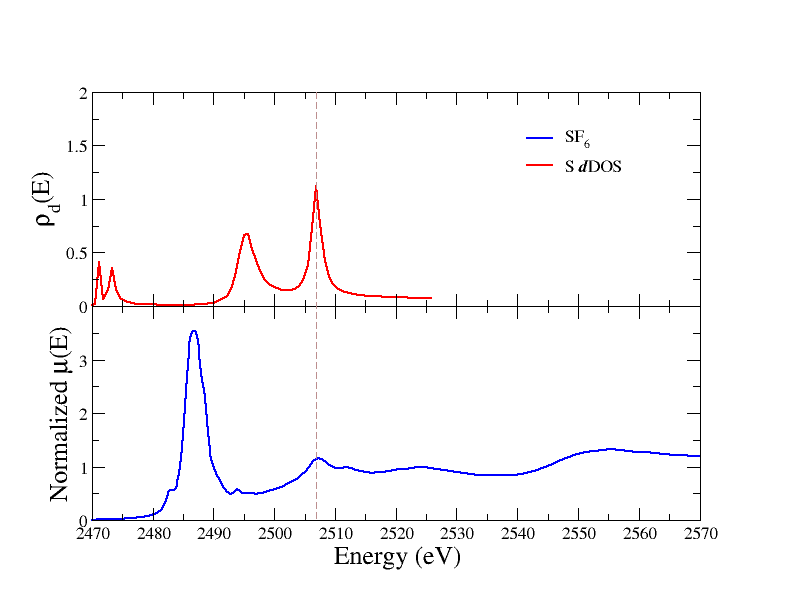
\includegraphics[width=0.9\linewidth]{images/SF6/ddos}
    \end{column}
    \begin{column}{6cm}
      SF$_6$ is an octahedral complex with nominal bond length of
      1.54\,\AA.  A distortion will mix \textit{p} and \textit{d}
      character in the final state with the peak near 2507\,eV in the
      \textit{d}DOS contributing spectrum.
      \begin{itemize}
      \item Thermal: $\langle R_{S,F_x} - R_{S,F_{-x}}\rangle \ne 0$
      \item Jahn-Teller
      \end{itemize}

      \medskip

      \centering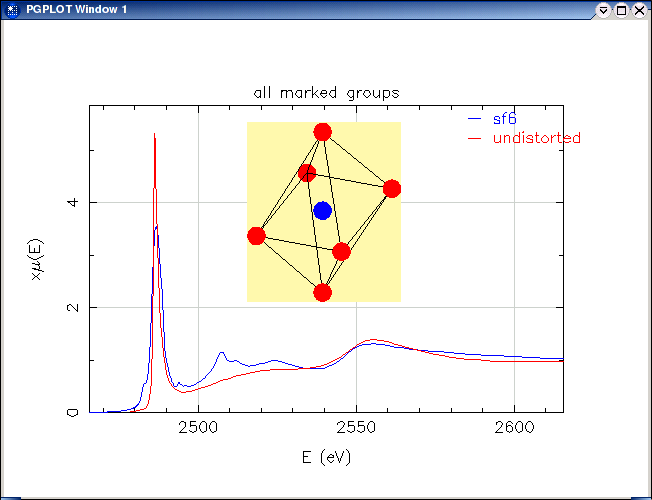
\includegraphics[width=0.86\linewidth]{images/SF6/sf6_undistorted}
    \end{column}
  \end{columns}
\end{frame}

\begin{frame}
  \frametitle{Self consistent potentials}

  \textsc{feff} starts with the potentials of the free atoms,
  $\rho_0(E)$.  It loops through the following calculations until
  the $\rho(E)$ functions stop changing.
  {\color{Blue4}
    \begin{equation*}
      \rho_\ell(E) = \rho_{0,\ell}(E)  \big(1 + \chi_\ell(E)\big)
      \qquad \ell \in \{0, 1, 2, 3, \cdots\}
    \end{equation*}
    }

  \begin{block}{Self consistency loop}
    \begin{equation*}
      \begin{CD}
        \rho_0(E) @>>> F(E),\Phi(E) @>>> \chi(E) \\
        && @AAA @VVV \\
        && \mathrm{converged?} @<<< \rho(E)
      \end{CD}
    \end{equation*}
  \end{block}

  \begin{center}
    At the end, $\rho(E)$ is integrated in energy.  The Fermi energy
    is where the integral equals the total number of valence electrons
    among the original free atoms in the cluster.  This integral also
    determines charge transfer.
  \end{center}
\end{frame}

\begin{frame}
  \frametitle{Fitting XANES spectra: Direct calculation}

  Compute XANES as a multivariate function of a large parameter space:
  \begin{definition}[Computed absorption]
    \centering$\mu(E,x_i,\alpha_j,\beta_k)$
  \end{definition}

  \begin{description}
    \item[$x_i$] the positions of all atoms in the cluster
    \item[$\alpha_j$]  parameters of the potentials model (muffin
      tin radii, loss terms, the Fermi energy, etc)
    \item[$\beta_k$] empirical parameters (broadening, $E_0$, offset
      function, etc)
  \end{description}


  \begin{block}{Fitting loop}
    \begin{equation*}
      \begin{CD}
        \mu_{\mathrm{init}}(E, x_i, \alpha_j, \beta_k) @>>>
        \mathrm{compare~to~data} @>>> \mathrm{adjust}~ x_i, \alpha_j, \beta_k \\
        && @AAA @VVV \\
        && \mu_{\mathrm{refined}}(E, x_i, \alpha_j, \beta_k) @<<< \mathrm{converged?}
      \end{CD}
    \end{equation*}
  \end{block}

  In the \textsc{feff} world, this is an open problem.  But see, for
  example, MXAN by M.\ Benfatto et al. PRB \textbf{65} (2002) 174205.
\end{frame}

\begin{frame}
  \frametitle{Fitting XANES spectra: multidimensional interpolation approximation}

  \begin{itemize}
  \item Another approach to the fitting XANES data is to precompute
    an adequate grid in the parameters $x_i$, $\alpha_j$, and
    $\beta_k$ and to place the data within that grid by
    multidimensional interpolation.
  \item This approach is quick after the initial computational expense.
  \item This has been implemented as the program \textsc{FitIt} by
    Grigory Smolentsev and Alexander V. Soldatov.  See
    \href{http://xafs.org/Software/FitIt}{\color{Purple4}\texttt{http://xafs.org/Software/FitIt}}
  \end{itemize}
\end{frame}

%%% Local Variables:
%%% mode: latex
%%% TeX-master: "pimst2"
%%% End:
